% Author: David Larsen <dcl9934@cs.rit.edu>
% Author: Doug Krofcheck <dpk3062@rit.edu>
\documentclass[11pt]{article}
\usepackage{fullpage}   %
\usepackage{listings}   %
\usepackage{needspace}  %
\usepackage{color}      %
\usepackage{ifthen}     % 
\usepackage{graphicx}   %
\usepackage{csc}        %
\usepackage{tikz}       %
\usetikzlibrary{shapes} %
\usepackage{tabularx}   % for helping matchtabular (matching questions)
\usepackage{textcomp}	% So our quotes in code don't look like shit
\usepackage{longtable}

\lstset{ %
basicstyle=\footnotesize\ttfamily,       % the size of the fonts that are used for the code
numbers=left,                   % where to put the line-numbers
stepnumber=1,                   % the step between two line-numbers. If it's 1 each line will be numbered
numbersep=5pt,                  % how far the line-numbers are from the code
showspaces=false,               % show spaces adding particular underscores
showstringspaces=false,         % underline spaces within strings
tabsize=4,		                % sets default tabsize to 4 spaces
language=Java,
upquote=true,
columns=fixed
}

\ifthenelse{\isundefined{\isAnswerKey}}
{
    \newenvironment{answer}{\large\lstset{basicstyle=\large\ttfamily}\color{white} \small{Answer:}\large}{}
}
{
    \newenvironment{answer}{\large\lstset{basicstyle=\large\ttfamily}\color{red} \small{Answer:}\large}{}
}

% ----- Start matchtabular definition -----
\newcounter{matchleft}
\newcounter{matchright}
\newenvironment{matchtabular}{%
  \setcounter{matchleft}{0}%
  \setcounter{matchright}{0}%
  \tabularx{\textwidth}{%
    >{\leavevmode\hbox to 1.5em{\stepcounter{matchleft}\arabic{matchleft}.}}X%
    >{\leavevmode\hbox to 1.5em{\stepcounter{matchright}\alph{matchright})}}X% 
    }%
}{\endtabularx}
% ----- End matchtabular definition -----

\title{CSCI-142 Midterm Exam Review}
\author{Computer Science Community}
\date{\today}

\makeatletter
\let\thetitle\@title
\let\theauthor\@author
\let\thedate\@date
\makeatother

\begin{document}
\header
\begin{enumerate}



\item Provide a detailed explaination of what the following code does:
\begin{lstlisting}
public boolean checkString(String a, String b) {
	return a == b;
}
\end{lstlisting}
\begin{answer}
Given the two strings $a$ and $b$, checkString() returns true if both string objects have the same memory address.  That means they are both references to the same thing.  The function does not check to see if the two strings have the same string value.  It is possible for two different strings to have the same value (``hellos'') but with different memory addresses.  

Talk about how, by default, Object's equal() checks memory addresses and can be extended by subclasses to check the objects' attributes.  In Java, it is not possible to override how == works.

To check if the contents of the strings are the same, use the {\tt equals} method, defined in the {\tt Object} class and overridden in the {\tt String} class.
For example, {\tt "yes".equals("yes")}.
\end{answer}



\item If an instance variable is declared with {\tt protected} access, who can access it? \\
\begin{answer}
Any class in the same package as the class in which the variable is defined.
\end{answer}



\item What is the difference between overriding and overloading methods?  Give a example situation where each should be used. \\
\begin{answer}
\textbf{Overriding:} method with the exact same method declaration as a method in a superclass; overwrites and/or extends the functionality of the super() method.

\textbf{Overloading:} 2 or more methods with the same name and return type that either:
	\begin{enumerate}
	\item have a different number of parameters\\ \textbf{OR}
	\item have parameters of different types
	\end{enumerate}
Override a method when you want to REPLACE the implementation of a method in a superclass.  Overload a method (such as a constructor) when you want to have more than one implementation of a method for different circumstances.
\end{answer}



\item Explain the differences between:
\begin{enumerate}
	\item class vs object \\
	\begin{answer}
	A class defines methods and fields---it can be viewed as a template. An object is an instance of a class. Think of classes as molds and objects as individual things created by those molds.
	\end{answer}	
	
	\item constant vs non-constant field (variable).  Declare a constant varable. \\
	\begin{answer}
	A constant field cannot be change during run time (it may be set {\em once}).
		\begin{lstlisting}[numbers=none]
public final int NUM_PEOPLE_WHO_LIKE_JAVA = 1;
		\end{lstlisting}
	\end{answer}
	
	\item constant vs non-constant method.  \\
	\begin{answer}
	A constant method cann't be overridden by a subclass.
	\end{answer}

	\item class vs instance variable.  Declare variables of both types.\\
	\begin{answer}
	Class (static) variables are scoped to their class not to an object.  All instances of a class access the same static variable.  Each class instance can only reference it's own instance (non-static) variable.
		\begin{lstlisting}[numbers=none]
class Types {
	public static int im_a_class_var = 1;
	public int im_an_instance_var = 2;
}
		\end{lstlisting}
	\end{answer}
	
	\item open addressing vs chaining \\
	\begin{answer}
	When a hash collision occurs, open addressing puts the new element in the next empty slot while chaining adds the new element to a list in the collided slot.  
	\end{answer}
\end{enumerate}



\item Define polymorphism and explain a situation in which you would use it. \\
\begin{answer}
Polymorphism: the ability to create an object of more than one type. References and collections of a super class may hold instances of subclasses. Methods invoked on these objects determine the correct (type specific) behavior at runtime. \\
EX:
		\begin{lstlisting}
ArrayList<Shape> shapes = new ArrayList<Shape>();

// Square with side length of 1
shapes.add(new Square(1.0));

// Circle with radius of 9
shapes.add(new Circle(9.0));

// Triangle with base of 4 and height of 5
shapes.add(new Triangle(4.0, 5.0));

// Outputs the correct area of each shape
for( int i = 0; i < shapes.size(); i++ ){ 
   	double area = shapes.get(i).getArea();
   	System.out.println(area);
}
        \end{lstlisting}
\end{answer}



\item What is the difference between an abstract class and an interface? Why might you want to use an interface over an abstract class? \\
\begin{answer}
Abstract classes allow for default method behavior to be defined, while interfaces allow only method declaration.  Since Java allows a class to extend only a single class but implement many interfaces, interfaces provide some extended capabilities. However, extending an abstract class allows usage of the defined default behaviors. 
\end{answer}


\newpage


\item What gets printed by the following code?
\begin{lstlisting}
public class Class1 {
	public Class1() {
		System.out.println( "Class1()" );
	}
	public void print1() {
		System.out.println( "Class1.print1()" );
	}
	public void print2() {
		System.out.println("Class1.print2()" );
	}
}

public class Class2 extends Class1 {
	public Class2() {
		System.out.println( "Class2()" );
	}
	public void print1() {
		System.out.println("Class2.print1()");
	}
}

public class Class3 extends Class1{
	private Class2 class2;
	public Class3() {
		System.out.println( "Class3()" );
		class2 = new Class2();
	}
	public void print1() {
		class2.print1();
	}
	public void print2(){
		System.out.println("Class3.print2()");
		super.print2();
	}
}

public class TestClass {
	public static void main( String[] args ) {
		Class1 c1 = new Class2();
		c1.print1();
		c1.print2();

		System.out.println();
		Class1 c2 = new Class3();
		c2.print1();
		c2.print2();
	}
}
\end{lstlisting}
\begin{answer}
    \begin{verbatim}
Class1()
Class2()
Class2.print1()
Class1.print2()

Class1()
Class3()
Class1()
Class2()
Class2.print1()
Class3.print2()
Class1.print2()
    \end{verbatim}
\end{answer}


\newpage


\item Find at least 3 errors related to inheritance and interfaces in the following code:\label{demolition-derby}
\begin{lstlisting}
public interface Vehicle {
	public int getSpeed();
	public void accelerate(int speed_increase);
	public void brake(int speed_decrease);
}
public class Car implements Vehicle {
	private int speed;
	public Car(int initialSpeed){
		this.speed = initialSpeed;
	}
	public int getSpeed(){
		return speed;
	}
	public int accelerate(int speed_increase) {
		speed += speed_increase;
	}
	public int brake(int speed_decrease) {
		speed -= speed_decrease;
	}
}
public class Toyota extends Car {
	public long getSpeed(){
		return speed;
	}
	public void brake(Integer speed_decrease) {}
	public void factoryRecall(){
		System.out.println("Replace my floor mat!");
	}
}
public class Truck implements Vehicle {
	public void accelerate(int speed_increase) {
		super.accelerate(speed_increase/2);
	}
	public void brake(int speed_decrease) {
		super.brake(speed_decrease/2);
	}
}
public class demolitonDerby {
	public static void main(String[] args) {
		Vechicle	prius, mack, impreza;
		prius = new Toyota();
		mack = new Truck();
		impreza = new Car();
		
		impreza.accelerate(5);
		prius.brake(2);
		prius.factoryRecall();
		prius.accelerate(impreza.getSpeed());
		mack.accelerate(5.0);
	}
\end{lstlisting}
\begin{answer}
    \begin{tabular}{r l} % TODO Fix some answers here
    Line \# & Error \\\hline
    14  	& Returns int, should return void\\
    17  	& Returns int, should return void\\
    22  	& getSpeed()'s return type ({\tt long}) differs from Car or Vehicle.\\
    23  	& speed is private.\\
    25,46	& Calling brake() on Toyotas will call the superclass's brake()\\
    30  	& Truck implements vehicle, but does not have getSpeed()\\
    32  	& Can't call super(), this has no superclass.\\
    33  	& Can't call super(), this has no superclass.\\
    47  	& {\tt prius} was declared as a {\tt Vehicle}, so we can't call\\
    ~  		& methods that aren't declared in {\tt Vehicle}.\\
    49  	& FIXME I don't think it's legal to pass a double to an int without casting.
    \end{tabular}
\end{answer}


\section*{Sorting}


\item Fill in the table for the asymptotic running time of each sorting algorithm.
\begin{center}
	\begin{tabular}{|r|c|c|c|} \hline
	~ & Best & Worst & Average \\\hline
	MergeSort &
		\begin{answer}$O(n*\textrm{log}(n))$\end{answer} &
		\begin{answer}$O(n*\textrm{log}(n))$\end{answer} &
		\begin{answer}$O(n*\textrm{log}(n))$\end{answer} \\\hline
	Quicksort &
		\begin{answer}$O(n*\textrm{log}(n))$\end{answer} &
		\begin{answer}$O(n^2)$\end{answer} &
		\begin{answer}$O(n*\textrm{log}(n))$\end{answer} \\\hline
	HeapSort &
		\begin{answer}$O(n*\textrm{log}(n))$\end{answer} &
		\begin{answer}$O(n*\textrm{log}(n))$\end{answer} &
		\begin{answer}$O(n*\textrm{log}(n))$\end{answer} \\\hline
	\end{tabular}
\end{center}



\item Match the partial algorithm descriptions \\
\begin{matchtabular}
Mergesort & Elements are taken out of a built data structure one at a time and placed in their proper location.\\
Quicksort & Splits its input into two other lists by always breaking the input in half.\\
Heapsort  & Splits its input into two (or three) other lists. One list's elements are smaller than a chosen value and another list's elements are larger than the chosen value. \\
\end{matchtabular}
\begin{answer}
	\begin{tabular}{l l}
	1. Megresort & b\\
	2. Quicksort & c\\
	3. Heapsort  & a\\
	\end{tabular}
\end{answer}



\item When under what conditions does Quicksort hit it's worst-case time complexity and why? \\
\begin{answer}
When the data is (nearly) sorted and you always pick the first pivot (i.e. when the chosen pivot only and always reduces the list by itself).

Quicksort splits its input into two lists based on the value of the pivot.  If the pivot is either the smallest or the largest element, then one list will have no elements while the others have the rest of the elements. Deminstrated by the following substitution trace:
	\begin{verbatim}
	qsort([1,2,3,4])
	qsort([]) + [1] + qsort([2,3,4])
	qsort([]) + [1] + qsort([]) + [2] + qsort([3,4])
	qsort([]) + [1] + qsort([]) + [2] + qsort([]) + [3] + qsort([4])
	qsort([]) + [1] + qsort([]) + [2] + qsort([]) + [3] + qsort([4])
	qsort([]) + [1] + qsort([]) + [2] + qsort([]) + [3] + qsort([]) + [4] + qsort([])
	[1,2,3,4]
	\end{verbatim}
\end{answer}



\item How can we prevent Quicksort from hitting it's worst-case time complexity? \\
\begin{answer}
With real-world data, we're more likely to encounter ordered or semi-ordered data than randomised data. This makes it more likely for us run into Quicksort's worst-case time complexity. We run into this bad time complexity if we select pivots which are near the lowest or highest values.

Selecting a random pivot helps encounter the average case and thus evens out the distribution of ordered and unordered data. Even when we're given sorted data, if we select pivots randomly, we should be able to end up with average time complexity.

To guarantee non-worst-case complexity, pick the pivot using median-of-medians.  You'll learn about that in Analysis of Algorithms.
\end{answer}


\pagebreak


\item Using list [3,5,1,3,2,7,9], trace through the following algorithms.  Be sure to identify your pivot(s). \\
\begin{enumerate}
	\item Mergesort \\
	\begin{answer}

		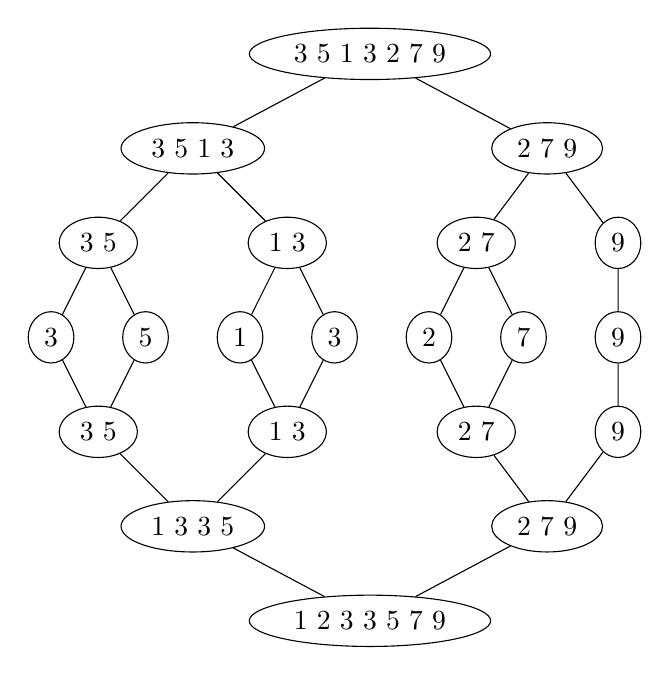
\begin{tikzpicture}[scale=1.2]
		\node [draw,ellipse] at (3.375,3) (head) {3 5 1 3 2 7 9};
		\node [draw,ellipse] at (1.5,2) (1) {3 5 1 3};
		\node [draw,ellipse] at (5.25,2) (2) {2 7 9};
		\node [draw,ellipse] at (.5,1) (3) {3 5};
		\node [draw,ellipse] at (2.5,1) (4) {1 3};
		\node [draw,ellipse] at (4.5,1) (5) {2 7};
		\node [draw,ellipse] at (6,1) (6) {9};
		\node [draw,ellipse] at (0,0) (7) {3};
		\node [draw,ellipse] at (1,0) (8) {5};
		\node [draw,ellipse] at (2,0) (9) {1};
		\node [draw,ellipse] at (3,0) (10) {3};
		\node [draw,ellipse] at (4,0) (11) {2};
		\node [draw,ellipse] at (5,0) (12) {7};
		\node [draw,ellipse] at (6,0) (13) {9};
		\node [draw,ellipse] at (.5,-1) (14) {3 5};
		\node [draw,ellipse] at (2.5,-1) (15) {1 3};
		\node [draw,ellipse] at (4.5,-1) (16) {2 7};
		\node [draw,ellipse] at (6,-1) (17) {9};
		\node [draw,ellipse] at (1.5, -2) (18) {1 3 3 5};
		\node [draw,ellipse] at (5.25, -2) (19) {2 7 9};
		\node [draw,ellipse] at (3.375,-3) (20) {1 2 3 3 5 7 9};

		\path [draw] (1) -- (head) -- (2);
		\path [draw] (3) -- (1) -- (4);
		\path [draw] (5) -- (2) -- (6);
		\path [draw] (7) -- (3) -- (8);
		\path [draw] (9) -- (4) -- (10);
		\path [draw] (11) -- (5) -- (12);
		\path [draw] (13) -- (6);
		\path [draw] (7) -- (14) -- (8);
		\path [draw] (9) -- (15) -- (10);
		\path [draw] (11) -- (16) -- (12);
		\path [draw] (13) -- (17);
		\path [draw] (14) -- (18) -- (15);
		\path [draw] (16) -- (19) -- (17);
		\path [draw] (18) -- (20) -- (19);
		\end{tikzpicture}\\*
	\end{answer}

	\item Quicksort \\
	\begin{answer}
	(using the first element in the list as a pivot)\\*
		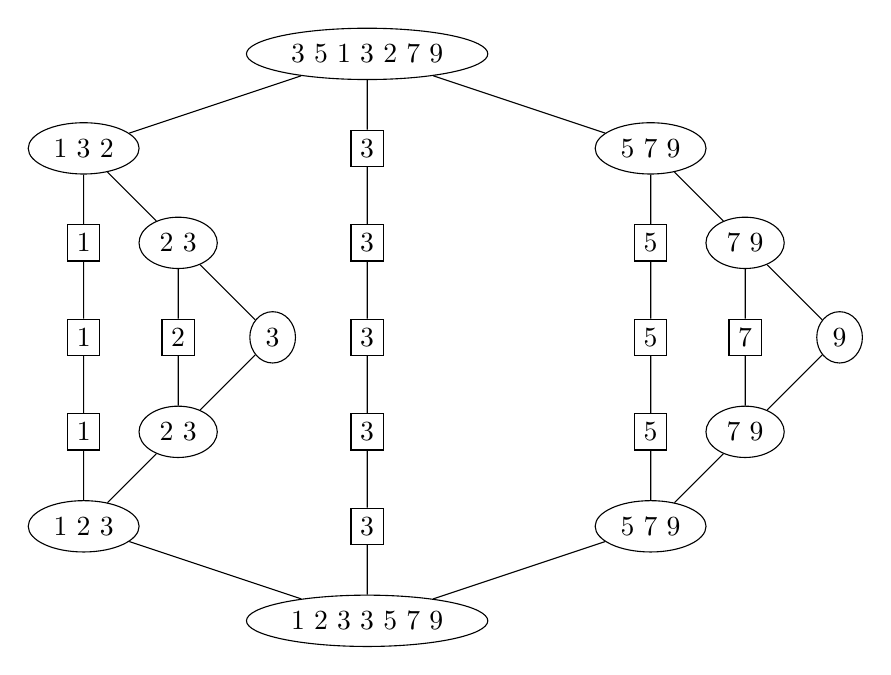
\begin{tikzpicture}[scale=1.2]
		\node [draw] at (1,0) (1) {1};
		\node [draw] at (2,0) (2) {2};
		\node [draw,ellipse] at (3,0) (3) {3};
		\node [draw] at (4,0) (4) {3};
		\node [draw] at (7,0) (5) {5};
		\node [draw] at (8,0) (6) {7};
		\node [draw,ellipse] at (9,0) (7) {9};
		\node [draw] at (1,1) (8) {1};
		\node [draw, ellipse] at (2,1) (9) {2 3};
		\node [draw] at (4,1) (10) {3};
		\node [draw] at (7,1) (11) {5};
		\node [draw,ellipse] at (8,1) (12) {7 9};
		\node [draw, ellipse] at (1,2) (13) {1 3 2};
		\node [draw] at (4,2) (14) {3};
		\node [draw,ellipse] at (7,2) (15) {5 7 9};
		\node [draw,ellipse] at (4,3) (16) {3 5 1 3 2 7 9};
		\node [draw] at (1,-1) (17) {1};
		\node [draw,ellipse] at (2,-1) (18) {2 3};
		\node [draw] at (4, -1) (19) {3};
		\node [draw] at (7,-1) (20) {5};
		\node [draw, ellipse] at (8,-1) (21) {7 9};
		\node [draw, ellipse] at (1,-2) (22) {1 2 3};
		\node [draw] at (4,-2) (23) {3};
		\node [draw, ellipse] at (7,-2) (24) {5 7 9};
		\node [draw, ellipse] at (4,-3) (25) {1 2 3 3 5 7 9};

		\path [draw] (1) -- (8) -- (13);
		\path [draw] (2) -- (9);
		\path [draw] (3) -- (9) -- (13);
		\path [draw] (4) -- (10) -- (14) -- (16);
		\path [draw] (5) -- (11) -- (15);
		\path [draw] (6) -- (12);
		\path [draw] (7) -- (12) -- (15) -- (16);
		\path [draw] (13) -- (16);

		\path [draw] (1) -- (17) -- (22);
		\path [draw] (2) -- (18);
		\path [draw] (3) -- (18) -- (22) -- (25);
		\path [draw] (4) -- (19) -- (23) -- (25);
		\path [draw] (5) -- (20) -- (24);
		\path [draw] (6) -- (21);
		\path [draw] (7) -- (21) -- (24) -- (25);
		\end{tikzpicture}
	\end{answer}

	\item Heapsort (show heap creation too)\\
	\begin{answer}
		Heapify: \\
			\begin{longtable}{c l}
			Tree Heap & Array Heap\\
			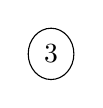
\begin{tikzpicture}[scale=1]
				\node [draw, ellipse] at (0,0) {3};
			\end{tikzpicture} &
			[\underline{3}, 5, 1, 3, 2, 7, 9] \\

			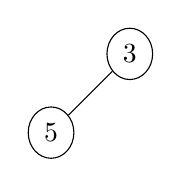
\begin{tikzpicture}[scale=1]
				\node [draw, ellipse] at (0,0) (3) {3};
				\node [draw, ellipse] at (-1,-1) (5) {5};

				\path [draw] (3) -- (5);
			\end{tikzpicture} &
			[\underline{3}, \underline{5}, 1, 3, 2, 7, 9] \\

			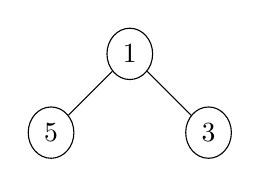
\begin{tikzpicture}[scale=1]
				\node [draw, ellipse] at (0,0) (1) {1};
				\node [draw, ellipse] at (-1,-1) (5) {5};
				\node [draw, ellipse] at (1,-1) (3) {3};

				\path [draw] (1) -- (5);
				\path [draw] (1) -- (3);
			\end{tikzpicture} &
			[\underline{1}, \underline{5}, \underline{3}, 3, 2, 7, 9] \\

			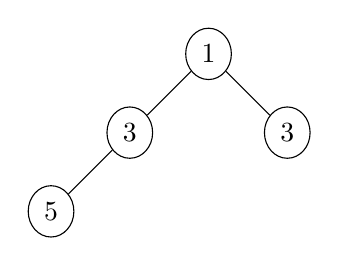
\begin{tikzpicture}[scale=1]
				\node [draw, ellipse] at (0,0) (1) {1};
				\node [draw, ellipse] at (-1,-1) (3) {3};
				\node [draw, ellipse] at (1, -1) (31) {3};
				\node [draw, ellipse] at (-2, -2) (5) {5};

				\path [draw] (1) -- (3) -- (5);
				\path [draw] (1) -- (31);
			\end{tikzpicture} &
			[\underline{1}, \underline{3}, \underline{3}, \underline{5}, 2, 7, 9] \\


			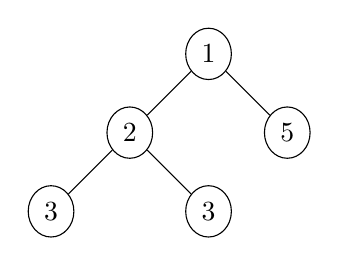
\begin{tikzpicture}[scale=1]
				\node [draw, ellipse] at (0,0) (1) {1};
				\node [draw, ellipse] at (-1,-1) (2) {2};
				\node [draw, ellipse] at (1, -1) (5) {5};
				\node [draw, ellipse] at (-2, -2) (3) {3};
				\node [draw, ellipse] at (0, -2) (31) {3};

				\path [draw] (1) -- (2) -- (3);
				\path [draw] (1) -- (5);
				\path [draw] (2) -- (31);
			\end{tikzpicture} &
			[\underline{1}, \underline{2}, \underline{5}, \underline{3}, \underline{3}, 7, 9] \\


			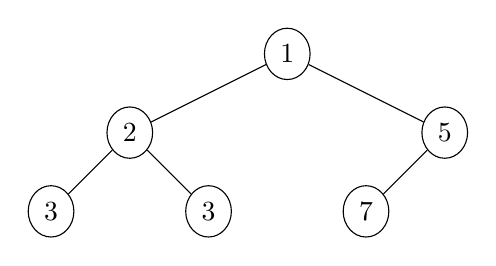
\begin{tikzpicture}[scale=1]
				\node [draw, ellipse] at (0,0) (1) {1};
				\node [draw, ellipse] at (-2,-1) (2) {2};
				\node [draw, ellipse] at (2, -1) (5) {5};
				\node [draw, ellipse] at (-3, -2) (3) {3};
				\node [draw, ellipse] at (-1, -2) (31) {3};
				\node [draw, ellipse] at (1, -2) (7) {7};

				\path [draw] (1) -- (2) -- (3);
				\path [draw] (1) -- (5);
				\path [draw] (2) -- (31);
				\path [draw] (5) -- (7);
			\end{tikzpicture} &
			[\underline{1}, \underline{2}, \underline{5}, \underline{3}, \underline{3}, \underline{7}, 9] \\

			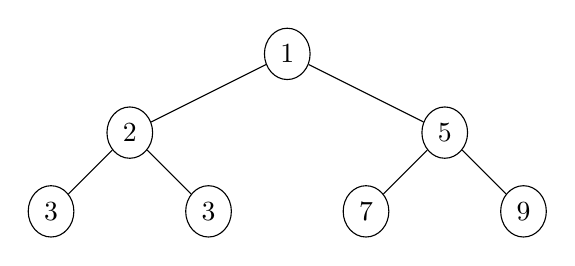
\begin{tikzpicture}[scale=1]
				\node [draw, ellipse] at (0,0) (1) {1};
				\node [draw, ellipse] at (-2,-1) (2) {2};
				\node [draw, ellipse] at (2, -1) (5) {5};
				\node [draw, ellipse] at (-3, -2) (3) {3};
				\node [draw, ellipse] at (-1, -2) (31) {3};
				\node [draw, ellipse] at (1, -2) (7) {7};
				\node [draw, ellipse] at (3, -2) (9) {9};

				\path [draw] (1) -- (2) -- (3);
				\path [draw] (1) -- (5);
				\path [draw] (2) -- (31);
				\path [draw] (5) -- (7);
				\path [draw] (5) -- (9);
			\end{tikzpicture} &
			[\underline{1}, \underline{2}, \underline{5}, \underline{3}, \underline{3}, \underline{7}, \underline{9}] \\
			\end{longtable}

		Sort: \\
			\begin{longtable}{c l}
			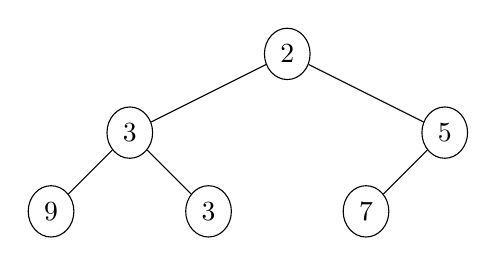
\begin{tikzpicture}[scale=1]
				\node [draw, ellipse] at (0,0) (1) {2};
				\node [draw, ellipse] at (-2,-1) (2) {3};
				\node [draw, ellipse] at (2, -1) (5) {5};
				\node [draw, ellipse] at (-3, -2) (3) {9};
				\node [draw, ellipse] at (-1, -2) (31) {3};
				\node [draw, ellipse] at (1, -2) (7) {7};

				\path [draw] (1) -- (2) -- (3);
				\path [draw] (1) -- (5);
				\path [draw] (2) -- (31);
				\path [draw] (5) -- (7);
			\end{tikzpicture} &
			[\underline{2}, \underline{3}, \underline{5}, \underline{9}, \underline{3}, \underline{7}, 1] \\

			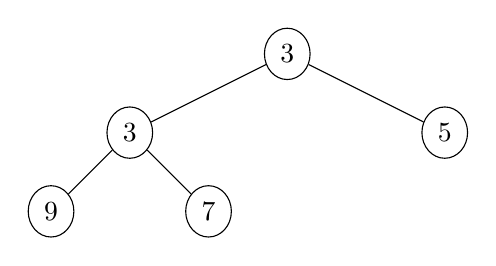
\begin{tikzpicture}[scale=1]
				\node [draw, ellipse] at (0,0) (1) {3};
				\node [draw, ellipse] at (-2,-1) (2) {3};
				\node [draw, ellipse] at (2, -1) (5) {5};
				\node [draw, ellipse] at (-3, -2) (3) {9};
				\node [draw, ellipse] at (-1, -2) (31) {7};

				\path [draw] (1) -- (2) -- (3);
				\path [draw] (1) -- (5);
				\path [draw] (2) -- (31);
			\end{tikzpicture} &
			[\underline{3}, \underline{3}, \underline{5}, \underline{9}, \underline{7}, 2, 1] \\

			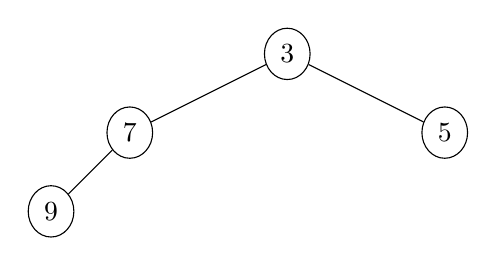
\begin{tikzpicture}[scale=1]
				\node [draw, ellipse] at (0,0) (1) {3};
				\node [draw, ellipse] at (-2,-1) (2) {7};
				\node [draw, ellipse] at (2, -1) (5) {5};
				\node [draw, ellipse] at (-3, -2) (3) {9};

				\path [draw] (1) -- (2) -- (3);
				\path [draw] (1) -- (5);
			\end{tikzpicture} &
			[\underline{3}, \underline{7}, \underline{5}, \underline{9}, 3, 2, 1] \\

			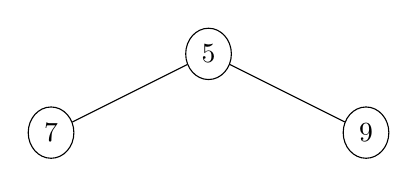
\begin{tikzpicture}[scale=1]
				\node [draw, ellipse] at (0,0) (1) {5};
				\node [draw, ellipse] at (-2,-1) (2) {7};
				\node [draw, ellipse] at (2, -1) (5) {9};

				\path [draw] (1) -- (2);
				\path [draw] (1) -- (5);
			\end{tikzpicture} &
			[\underline{5}, \underline{7}, \underline{9}, 3, 3, 2, 1] \\

			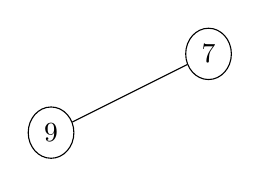
\begin{tikzpicture}[scale=1]
				\node [draw, ellipse] at (0,0) (1) {7};
				\node [draw, ellipse] at (-2,-1) (2) {9};

				\path [draw] (1) -- (2);
			\end{tikzpicture} &
			[\underline{7}, \underline{9}, 5, 3, 3, 2, 1] \\

			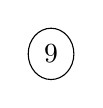
\begin{tikzpicture}[scale=1]
				\node [draw, ellipse] at (0,0) (1) {9};
			\end{tikzpicture} &
			[\underline{9}, 7, 5, 3, 3, 2, 1] \\

			&
			[9, 7, 5, 3, 3, 2, 1] \\
			\end{longtable}
	\end{answer}
\end{enumerate}



\section*{Heaps and Heapsort} %TODO remove this and create better section headers (assuming we're keeping headers)



\item For a binary heap containing $n$ elements, what is the maximum number of swaps occurring after an insert operation? \\
\begin{answer}
$\log_2 (n + 1)$, rounded down.
\end{answer}



\item Given a node in an array-based binary heap at index $i$, where are the indices of both its children? What is the index of its parent? \\
\begin{answer}
The children are at $2i+1$ and $2i+2$. The parent is at $\lfloor\frac{i-1}{2}\rfloor$.

\marginpar{\small\em Note that in a 1 indexed array system, the children would be at $2i$ and $2i+1$.  The parent would be at $\lfloor\frac{i}{2}\rfloor$.} 
\end{answer}


\newpage
\section*{Hash Maps}


Dorothy started to write her own implementation of a hash map to store {\tt String}s and {\tt int}s, but before she finished she was carried away by flying monkeys who have a strong dislike for fast lookup times. Before her unfortunate departure she was able to write a {\tt LinkedNode} class which has data members {\tt key, value,} and {\tt next}, as well as the following code:
\begin{lstlisting}
import java.util.ArrayList;

public class DorothysHashMap {
	private ArrayList<LinkedNode> table;
	private int capacity;
    
	DorothysHashMap() {
		capacity = 100;
		table = new ArrayList<LinkedNode>(capacity);
		for (int i=0; i < table.size(); i++) {
			table.add(null);
		}
	}
    
	private int badHash( String key ) {
		return key.length() % capacity;
	}
    
	public void put( String key, int value ) {
		int hashIndex = badHash( key );
		if ( table.get( hashIndex ) == null ) {
			LinkedNode newNode = new LinkedNode( key, value, null );
			table.set( hashIndex, newNode );
		}
		else {
			LinkedNode current = table.get( hashIndex );
			while ( current.getNext() != null && !current.getKey().equals( key ) ) {
				current = current.getNext();
			}
			if ( current.getKey().equals( key ) ) {
				current.setValue( value );
			}
			else {
				LinkedNode newNode = new LinkedNode(key, value, null);
				current.setNext( newNode );
			}
		}
	}
}
\end{lstlisting}



\item Judging from her code, was {\tt DorothysHashMap} intended to use Chaining or Open Addressing to handle collisions? How can you tell? \\
\begin{answer}
Chaining. You can tell because there is a linked list stored in each index of the ArrayList.
\end{answer}



\item Assuming that Dorothy was intending to use English words as keys, is the hashing function she wrote a good one? Why or why not? \\
\begin{answer}
No, it uses the length of the input string while most English words are roughly the same length (probably less than 50 characters). We should take advantage of the individual values of the characters in the words, not the number of characters.  
\end{answer}



\item Dorothy also wrote the stub for the {\tt get()} method but didn't finish it. Complete the rest of it for her. You can return {\tt -1} if the key is not found in the hash map. \\
{\tt public int get( String key ) \{ } \\
\begin{answer} 
	\begin{lstlisting}
	int hashIndex = badHash( key );
	// if key is not in table, return -1
	if ( table.get( hashIndex ) == null ) {
		return -1;
	}
	LinkedNode current = table.get( hashIndex );
	while ( current.getNext() != null 
		&& !current.getKey().equals( key ) ) {
		current = current.getNext();
	}
	if ( current.getKey().equals( key) ) {
		return current.getValue();
	}
	else {
		// We looped thru the entire list and didn't find it
		return -1;
	}
}
	\end{lstlisting}
\end{answer}



\end{enumerate}
\end{document}

Note: The following numbers are outdated:

TODO: Generics-make the following code generic, ???

Topics for this exam:
	- Java basics
		1, 2, 3, 4
	- Classes
	- Inheritance (interfaces & subclasses)
		5?, 6, 7, 8, 9
	- O(NlogN) sorts... mergesort and quicksort
		10, 11, 12, 13, 14, 15
	- Hashing
	- Heaps
		16, 17, 18

1) == vs .equals()
2) protected variables
3) overriding vs overloading methods
4) class vs object, constants vs normal, class vs instance, open vs chaining
6) polymorphism
7) abstract class vs interface
8) "What gets printed by the following code?" ... branches of classes
9) Given code of inheritance/interfaces, find errors.
10) time complexity for different sort algorithms
11) quicksort, mergesort, heapsort definitions
12) quicksort time complexity, worst-case explanation
14) quicksort (pivot selection)
15) perform mergesort, quicksort, and heapsort on a given set of values
16) heap insertion
17) parent/child indeces in heap
18) run heapsort on given set of values
